\documentclass{article}

\usepackage{pgfplots}

\usepackage{tikz}
\usepackage{circuitikz}
\usepackage{graphicx}
\usepackage{float}


\begin{document}
\begin{titlepage}
\begin{center}
\line(1,0){300}\\
\huge{\bfseries MY FIRST REPORT }

\line(1,0){200}

 \end{center}
 \begin {center}
\textbf{E-BALL TECNOLOGY}
\begin{figure}[h]
\end{figure}
\end{center}
\centering
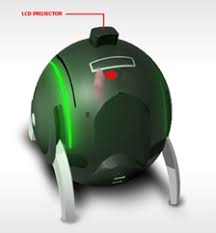
\includegraphics[height=0.3in]{index13.jpg}


    \begin{center}
        \vspace*{1cm}
       \textbf{Name:mouli afrin proma}
       
\begin{figure}[h]
\centering

\includegraphics[height=0.4in]{e-ball.jpg}

\end{figure}
 
        \Large
        \begin{flushleft}
        
         \textbf{  Computer Science and Engineering}
        \end{flushleft}
        
     
      
      \textbf{ID:18ICT CSE 033}
      
      \begin{flushleft}
             \textbf{ Shekh Hasina Institude of ICT Of Bangabandhu Sheikh Mujibor Rahman Science And Tecnolony University}
             \begin{figure}[h]
\centering

\includegraphics[height=0.7in]{bsmrstu.jpg}

\end{figure}
         
      \end{flushleft}

       \textbf{Gopalgonj,Bangladesh }
       
       
       \textbf{29/12/19}
 
 
    
    \end{center}
\end{titlepage}
\tableofcontents
\thispagestyle{empty}
\newpage
\textbf{A Review on E-Ball Technology}\\ 
1Deepa.B, 2Sri Bharathi.N and 3Tamilarasi.R, Department of Information Technology, Sri Krishna Arts and Science College, Coimbatore, Tamilnadu, India 
 
Abstract—The computer was invented in 19th century. The earlier computers are huge in size. Later on computers that are smaller than the ealier ones came into exist. But they are also space consuming. To avoid and manage this problem, innovative person creates the innovative hand-held computers with the properties of existing computers and with the improvised design.  This system is called as ‘e-ball’. It is a new concept of upcoming spherical shaped computers and laptops. This paper features about this new paradigm of e-ball technology which has all the features like traditional computer. Keywords—E-Ball, Spherical Shape, Virtual, Conventional, Paper Sheet Holder.\\

\newpage
\section{INTRODUCTION}
 
\textbf{I. INTRODUCTION: }\\


E-ball is  a emerging  technology which was invented 
by  a  31  year  old  Macedonian  product  designer,  Apostol 
Tnokovski. This is a new concept of PC which features all the 
traditional  elements  like  keyboard,  mouse,  webcam,  DVD 
player, projector  etc., and  it is the  smallest type  of computer 
ever made. It  is designed  to ease  the portability  and working 
without any hardware. Predominantly this concept is based on 
laser rays technique which dwells all the features of a computer. 
Principally it was  designed for  Microsoft Windows Operating 
System and it comprises of no external display units. This is the 
smallest model of this era.
 
When you close the e-ball no one can guess what is in 
that, that is none can find a whole computer set in that ball. But 
when  it  is  opened  we  can  see  a  whole  computer  set  which 
contains  all  the conventional  elements  like display  screen  as 
well as the virtual keyboard and a mouse. 
E-ball is designed to be placed on two stands and can 
be opened by simultaneously pressing the two buttons which is 
located on the  either side of the  sphere. It is provided  for the 
projection through LCD projector and navigation keys are given 
for  adjustment  purpose.  Because  of  its  unique  way,  e-ball 
computer has taken the computer technology to the peak.
\\


\begin{figure}[h]
\centering
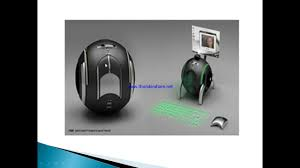
\includegraphics[height=2.5in]{index7.jpg}
\caption[optional caption]{E-Ballmodel}
\label{fig1: E-Ball model}


\end{figure}


 



\newpage
\section{COMPONENTS OF E-BALL}

\begin{figure}[h]
\centering
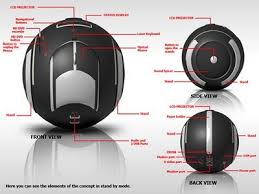
\includegraphics[height=2.5in]{index3.jpg}
\caption[optional caption]{Components in E-Ball model}
\label{fig2: E-Ball model}
\end{figure}


\newpage
 
\textbf{COMPONENTS OF E-BALL}
 \\
\textbf{A. Size Of Eball}
\\
 It is a spherical shaped ball of 6 inch in diameter and contains a motherboard of size 120x120mm.
 \\
 \textbf{B. Holographic Display}\\
  Holography is the best way of displaying the true 3Dimensional displays. It is a type of diffraction based display technology which reconstructs the light field of 3D in space with the coherent light. 
 
  \textbf{C. Processor}\\ 
  It has enhanced with dual core processor with two disassociated cores on the same die, providing its own cache.
  
   \textbf{D. Ram}\\
    RAM (Random Access Memory) is the dominant type of memory in the computer. This computer uses 5 Gigabytes of RAM. It gets the name because we can randomly access the memory without considering the sequence.
   \newpage
   \begin{figure}[h]
\centering
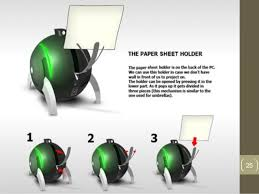
\includegraphics[height=2.5in]{index21.jpg}
\caption[optional caption]{E-Ball,model}
\label{fig1: E-Ball model}
\end{figure}
   \textbf{ E. Hard Disk Drive}\\
     It is a secondary storage device and non volatile in nature. It is made p of metal plate coated with oxide that is magnetized to store the digital information. Data can be directly accessed from the hard disk. This computer has the storage capacity in the range of 250-500 Gigabytes.
    
    \textbf{F. Speakers}\\
      Prominently known as multimedia speakers. It has two inbuilt 50W speakers.
     
    \textbf{G. HD DVD Recorder}\\
       High definition DVD recorder is an independent unit which dwells the functions of Video Cassette Recorder. It records into a DVD disc or in the internal disc.
      
   \textbf{H. Graphic Card And Sound Card}\\ 
      The graphic card is a hardware installed in the computer which is capable of generating output images on the screen. Almost all the modern motherboard consists of ports so that the graphic card can be embedded. The sound card is an integrated circuit which generates the sound which can be heard through the speakers.\\
 \textbf{I. Power Port And Modem Port}\\
  The power port is used to plug-in any electronic devices such as DVD player. The modem port is used to connect the internet to the computer. The computer uses the ISP (Internet Service Provider) to deliver the information.\\
  \textbf{ J. Webcam}\\
  The webcome is used vely used by all the computers. It can be connected to e-ball through USB cable or fire wire cable. K. Lan And Wan Cards LAN card is used to connect the users to Local Area Network through wireless connection. WAN card is a Network Interface Card which connects the user to a Wide Area Network.\\     
      
 \newpage 
 \section{WORKING OF E-BAL:}
 \textbf{WORKING OF E-BAL}\\
 works':





 E-ball concept of pc is a spherical shaped pc that grabs everyone’s attention. It is a modern system which doesn’t require any conventional keyboard and mouse. Here we discuss about the working of e-ball.\\
 
 \textbf{A.Lcd Projector}\\
 E-ball uses LCD (Liquid Crystal Display) Projectors to display or project the information on a flat surface. It consists of three LCD panels and each comprises of two glass panels with a layer of liquid crystals associated with them. It uses metal halide lamp to emit the light and a series of Di-chloric filters to separate the lights. Here the video signals are comprised of three colors: red, green and blue. These primary colors are making the images. LCD is generally more light efficient than DLP projectors. LCD projects the bright, vivid and sharper image with accurate color. This is the prominent advantage of LCD projector..\\
 \textbf{B. Dlp Projectors}\\
  DLP stands for Digital Light Processing. DLP technology is based on DMD (Digital Micromirror Device) chips. Each DMD chips is comprised of two million tiny mirrors. Each tiny mirror is capable of producing pixels. Color is fed to the DMD by a beam of light that passes through a spinning color wheels. Basic color wheels supports red, green and blue. After color reaches the DMD, the image is fed through the lens and onto the projection screen. The advantages of DLP projector are higher contrast and less door screen effect.\\ 
 \textbf{C.Optical Mouse}\\
  E-ball consists of optical wireless mouse which uses the concept of LED (Light emitting diode) and a light detector to detect the movements relative to a surface.\\
  \newpage
  \begin{figure}[h]
\centering
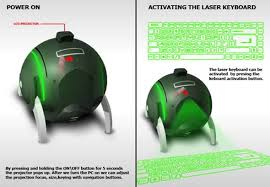
\includegraphics[height=2.5in]{index5.jpg}
\caption[optional caption]{Virtual Keyboard}
\label{fig1: E-Ball model}
\end{figure}
  \textbf{ D. Virtual Keyboard}\\
   It is a wireless laser projection keyboard which uses the principle of sensor technology. It is not a physical keyboard and it is interpreted through lasers. When the keyboard button is pressed, the keyboard is projected in the flat surface. Users have to touch the image of the key by moving the fingers through the air. Two technologies are used to transfer to the computer. In
   IJTRD | Jan-Feb 2017 Available Online@www.ijtrd.com \\ 
   \textbf{E. Paper Sheet}\\
    Holder Paper sheet holder can be used in the absence of walls. It is at the back of the pc. The lower part has to be pressed to open the paper sheet holder. The projector will recur by pressing the paper sheet holder button for five seconds. It is used to potrays the presentation.\\
    Figure 4: Paper-Sheet holder \\
    \newpage 
 \section{IV. NEEDS OF E-BALL :}
 \textbf{IV. NEEDS OF E-BALL :}\\
 The drawback of the earlier computers with heavy size and shape makes the use of the smallest e-ball computer.  The spherical shape of this computer is the best ever and can be carried to anywhere. It doesn’t need any space for physical monitor and other devices. As it is space consuming, it is the most preferable device to use.\\
\textbf{ International Journal of Trend in Research and Development, Volume 4(1), ISSN: 2394-9333 www.ijtrd.com }\\
\newpage
Figure 5: Scenarios of using E-ball \\
\begin{figure}[h]
\centering
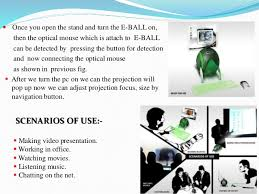
\includegraphics[height=2.5in]{index22.jpg}
\caption[optional caption]{ Seniors use of E-Ball tecnology}
\label{fig5: Seniors use of E-Ball tecnology}
\end{figure}
\textbf{Advantages of E-Ball}\\
  It is portable and it is hand free to use.\\
  It is efficient.\\
  It is more secured due to its shape.\\
  It has a larger storing capacity.\\ 
  It is easy to understand.\\
  It acquires high speed of execution.\\
  It is convenient for making presentations.\\
  \textbf{Disadvantages of E-Ball}
  Cost of e-ball is higher.\\
  It is not easy to understand if there is any error in the hardware resource.\\
  \newpage
  \section{V.CONCLUSION:}
               \textbf{CONCLUSION:}\\
  
   As the technology develops, the size of the computer is dwindling. Our imaginations are now coming true. The world has come to our pocket because of this device. The popularity of e-ball emphasizes the importance of technology. This e-ball concept of pc will move the world to the horizons.\\
     \newpage
     \section{VI.References:}
   \textbf{References}\\
   N. Ravi Bharti, J. Arul Jothi,\textbf{”E-Ball-A Complete Computer In A Ball”}, Dept of Master      of Computer Applications Sri Manakula Vinayagar Engineering College
  http://www.tuvie.com/e-ball-pc-concept-by-apostoltnokovski\\
  http://computers4you.blogspot.in/2009/03/review-e-ballpc-of-future.html\\
  http://www.google.co.in/EBALL \\
  http://www.electronics.howstuffworks.com\\
  
    \begin{tabular}{|c|c|c|c|}
    \hline
    Nafisa Zaman &Mouli Afrin &Israt Jahan &Zannatul Mim\\\hline
    id:01 &id:01 &id:03 &id:04\\\hline
    cgpa:2.55 &cgpa:3.55 &cgpa:4.00 &cgpa:3.78\\\hline
    \end{tabular}\\
  	[8 cm]
\subsection{Add Graph}
\begin{tikzpicture}[>=stealth]
    \begin{axis}[
        xmin=-4,xmax=4,
        ymin=-2,ymax=2,
        axis x line=middle,
        axis y line=middle,
        axis line style=<->,
        xlabel={$x$},
        ylabel={$y$},
        ]
        \addplot[no marks,blue,<->] expression[domain=-pi:pi,samples=100]{sin(deg(2*x))+1/2} 
                    node[pos=0.65,anchor=south west]{$y=\sin(2x)+\frac{1}{2}$}; 
    \end{axis}
\end{tikzpicture}
  
  
      
\end{document} 